%% Based on a TeXnicCenter-Template by Gyorgy SZEIDL.
%%%%%%%%%%%%%%%%%%%%%%%%%%%%%%%%%%%%%%%%%%%%%%%%%%%%%%%%%%%%%
%
%------------------------------------------------------------
%
\documentclass[a4paper,12pt,reqno]{article}
%----------------------------------------------------------
\usepackage{amsfonts}
\usepackage{listings}
\usepackage{graphicx}
\usepackage{geometry}
\usepackage{xcolor}
\usepackage{amssymb,amsmath}
\usepackage{polski}
\usepackage[T1]{fontenc}
\usepackage[utf8]{inputenc}
\usepackage{caption}
\geometry{margin=1.1in}
\usepackage{wrapfig}
\usepackage{lipsum}  
\usepackage{listings}
\usepackage[toc,page]{appendix}
\usepackage{url}
\usepackage{float}
\usepackage{amsmath}
\usepackage{indentfirst} % pierwszy akapit zawsze z wcięciem
\usepackage{subcaption}	% kilka zdjęc w jednej lini
\definecolor{codegreen}{rgb}{0.5, 0.09, 0.09}
\definecolor{codegray}{rgb}{0.5,0.5,0.5}
\definecolor{codepurple}{rgb}{0.58,0,0.82}
\definecolor{backcolour}{rgb}{0.94,0.94,0.94}
\definecolor{gray}{rgb}{0,0.6,0}

\lstdefinestyle{mystyle}{
    backgroundcolor=\color{backcolour},  
    commentstyle=\color{codegreen},
    keywordstyle=\color{blue},
    numberstyle=\tiny\color{codegray},
    stringstyle=\color{codepurple},
	basicstyle=\footnotesize\fontfamily{cmtt}\selectfont,
    breakatwhitespace=false,         
    breaklines=true,
    captionpos=b,
	language=C++,
    keepspaces=true,                 
    numbers=left,                    
    numbersep=5pt,                  
    showspaces=false,                
    showstringspaces=false,
    showtabs=false,                  
    tabsize=2
}

\lstset{style=mystyle}
\lstset{literate=%
    *{0}{{{\color{gray}0}}}1
    {1}{{{\color{gray}1}}}1
    {2}{{{\color{gray}2}}}1
    {3}{{{\color{gray}3}}}1
    {4}{{{\color{gray}4}}}1
    {5}{{{\color{gray}5}}}1
    {6}{{{\color{gray}6}}}1
    {7}{{{\color{gray}7}}}1
    {8}{{{\color{gray}8}}}1
    {9}{{{\color{gray}9}}}1
}
\lstset { %
    language=C++,
    backgroundcolor=\color{black!5}, % set backgroundcolor
    basicstyle=\footnotesize,% basic font setting
}
%------------------------------------------------------------
\begin{document}

%\begin{figure}[h]
%	\centering
%		
\includegraphics[width=0.40\textwidth]{logo.pdf}
%\end{figure}


\begin{center}

\thispagestyle{empty}

%UNIWERSYTET WROCŁAWSKI\\
\Large 
Uniwersytet Wrocławski\\
Wydział Fizyki i Astronomii\\
\vspace{0.8cm}
\vspace{1.8cm}

\Large Marcin Pietrzak \\
\vspace{3.2cm}
\Large Galeria modeli komputerowych \\
\vspace{1.5cm}
Computer models gallery
\end{center}
\vspace{3.7cm}
\begin{flushright}

\large{ Praca inżynierska na kierunku \\Informatyka Stosowana i Systemy Pomiarowe \\}
\vspace{0.5cm}
\large{ Opiekun \\ dr hab. Maciej Matyka, prof. UWr}
\end{flushright}
\vspace{2.2cm}

\begin{center}
\large Wrocław, \today
\end{center}

\newpage

\tableofcontents

\newpage

\begin{flushleft}
\Large \textbf{Streszczenie}
\end{flushleft}
\vspace{1cm}


 Lorem ipsum dolor sit amet, consectetur adipiscing elit, sed do eiusmod tempor incididunt ut labore et dolore magna aliqua. Ut enim ad minim veniam, quis nostrud exercitation ullamco laboris nisi ut aliquip ex ea commodo consequat. Duis aute irure dolor in reprehenderit in voluptate velit esse cillum dolore eu fugiat nulla pariatur. Excepteur sint occaecat cupidatat non proident, sunt in culpa qui officia deserunt mollit anim id est laborum.

\newpage
\begin{flushleft}
\Large \textbf{Abstract}
\end{flushleft}
\vspace{1cm}


Lorem ipsum dolor sit amet, consectetur adipiscing elit, sed do eiusmod tempor incididunt ut labore et dolore magna aliqua. Ut enim ad minim veniam, quis nostrud exercitation ullamco laboris nisi ut aliquip ex ea commodo consequat. Duis aute irure dolor in reprehenderit in voluptate velit esse cillum dolore eu fugiat nulla pariatur.

\newpage

\section{Wstęp}

\subsection{Wprowadzenie}

W pewnych aspektach życia człowiek zastanawia się nad paroma rzeczami, czy nie
jesteśmy sami w kosmosie, kiedy nastąpi koniec, czy VR umarł, czy nie jesteśmy
programem komputerowym. Pewnie nie poznamy odpowiedzi na te wszystkie
pytania, jeszcze przez jakiś czas, ale dzisiaj jedno jest pewne. VR na pewno jeszcze
nie umarł i ma się całkiem dobrze. W ciągu ostatnich kilku lat rynek gogli VR zaczął
na nowo się rozwijać, powstało wiele gogli, a do najpopularniejszych z nich należą:
PlayStation VR, Valve Index, HTC Vive Pro \cite{popularnosc_gogli}. Każde z tych gogli ma jednak wady, a
do najważniejszych należy to, że nie są to sprzęty typu plug and play. Trzeba się nie
tylko męczyć z splątaniną przewodów, ale także gogle jak np. Valve Index wymagają
stacji, dzięki którym gogle wiedzą gdzie znajdujesz się przestrzeni 3D. Kolejnym
problemem jest oczywiście cena samego sprzętu który w większości przekracza
ponad 3000 PLN za całość. Jedynie co się z tego zestawu różni to PlayStation VR,
same są jednak przestarzałe, a Sony zapowiedziało ich następcę którego premiera
nastąpi pod koniec 2022 roku \cite{PlayStation_VR2}. Same gogle Sony nie rozwiązały dla mnie
największego problemu, czyli obowiązek podłączenia przewodem, jednakże ten
problem na szczęście rozwiązała już inna firma, mowa oczywiście o Oculus znaną
obecnie jako Reality Labs, jedna z podfirm Facebooka obecnie znana jako Meta. Firma zaczęła
sprzedawać w 2019 gogle Oculus Quest, które były rewolucyjne z jednego ważnego
powodu, były autonomiczne, tzn. nie potrzebowały komputera do obsługi gogli,
ponieważ wystarczą do tego same gogle z kontrolerami ruchowymi. Same gogle nie
potrzebowały też stacji do określania położenia gogli, gdyż same w sobie mają diody
podczerwone które do tego służą. Oculus Quest okazał się dość rewolucyjnym
sprzętem wartym ok. 2000 pln za wersję podstawową, a rok później Oculus wypuścił
następcę za którego zapłaciliśmy jeszcze mniej czyli ok. 1500 pln w wersji
podstawowej. Nie odbyło się to bez kompromisów takich jak: Brak płynnej zmiany
rozstawu soczewek dla oczu, gorszej jakości pasek na głowę, brak magnetycznego
zabezpieczenia pojemnika na baterię. To nie znaczy oczywiścię, że gogle były
gorszę a do najważniejszych należą: Zwiększona roździelość obrazu dla jednego
oka, zmiana procesora na wydajniejszy, wydłużony czas pracy kontrolerów na jednej
baterii \cite{porownanie_gogli}. 

\begin{figure}[!ht]%
	\centering
	\begin{subfigure}{.5\textwidth}
		\centering
		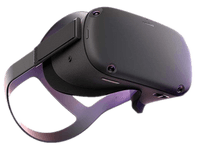
\includegraphics[width=0.8\linewidth]{graphics/oculusquest.png}
		\caption{Oculus Quest 1}	
		\label{ref:subref_a}
	\end{subfigure}%
	\begin{subfigure}{.5\textwidth}
		\centering
		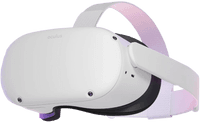
\includegraphics[width=0.8\linewidth]{graphics/oculusquest2.png}
		\caption{Oculus Quest 2}
		\label{ref:subref_b}
	\end{subfigure}%
	

\caption{Gogle VR od Oculusa}
\label{ref:ref}
\end{figure}

Quest 2 wśród gogli VR okazał się dużym sukcesem, w roku 2021
sprzedanych zostało 11,2 miliona sztuk urządzeń z czego 78\% to były Oculus Quest
2 \cite{Sprzedasz_gogli_VR}. Rynek aplikacji też się rozwinął w ciągu ostatnich lat. Na samego Oculusa Questa
w oficjalnym sklepie jest obecnie dostępnych ponad 300 aplikacji, na Steam jest ich
już ponad 2000. Oczywiście wśród nich nie znajdują się same gry, ponieważ gogle
mogą być wykorzystane też np. do zaprezentowania ciała człowieka, być platformą
do rysowania obrazów, lub sprzętem do relaksu czy oglądania filmów. Ja chciałem
spróbować swoich sił w stworzeniu małego projektu, który mógłby być wykorzystany
do pokazywania co ciekawego można robić w komputerze, czyli galerii modelów
komputerowych.

\begin{figure}[H]%
\centering
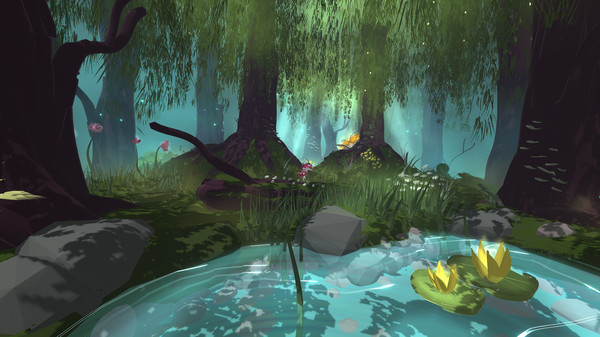
\includegraphics[width=0.8\columnwidth]{graphics/OpenBrush.png}
\caption{OpenBrush
\label{OpenBrush}}%
%
\qquad
\end{figure}  

\subsection{Cel i zakres pracy}

Głównym założeniem jest stworzenie aplikacji VR która przedstawi kilka wybranych
przeze mnie modeli komputerowych w przystępny sposób, łącznie z częścią galerii w
której znajdować się będzie historia danego modelu i ciekawostki z nim związane.
Gogle VR których używałem do testów to Oculus Quest pierwszej generacji,
natomiast aplikację napisałem w Unreal Engine 4, ponieważ mogę w tym silniku
pisać w języku C++, który to najbardziej z języków programowania znam, oraz w
blueprintach czyli Unrealowym wizualnym języku skryptowym, który jest przystępny
dla nowych użytkowników. Silnik posiada pełne wsparcie dla gogli VR czy to wersji
autonomicznej czy wersji PCVR. Sam aplikację pisałem z myślą o PCVR, ponieważ
nie musiałem się aż tak obawiać o ograniczenia które stawia sprzęt w wersji
androidowej np. brak wsparcia dla Unrealowych postprocesów obrazu. Projekt ten
pokazuję, że w dzisiejszych czasach dzięki dostępnym narzędziom typu UE4 i gogle
VR, człowiek jest w stanie stworzyć program w mało wymagający sposób który nie
byłby możliwy do zrealizowania jeszcze 10 lat temu.

\newpage
\section{Warstwa Użytkowa}

\subsection{Wygląd i Obsługa programu}
{\color{blue}
Program do uruchomienia wymaga gogli VR np. Oculus Quest i kontrolerów ruchowych. Można poruszać się po planszy na dwa sposoby. Pierwszy polega na użyciu lewego thumbsticka dzięki czemu można poruszać się płynnie po planszy, podczas poruszania się po planszy zmniejsza się obraz aby osoby które mają chorobę symulatorową\cite{choroba_vr} lepiej znosiły takie poruszanie się po poziomie. Drugi natomiast polega na teleportacji, po naciśnięciu przycisku B na prawy kontrolerze i wybraniu miejsca planszy gdzie chcemy się teleportować, jest to sposób poruszania się bardziej przyjazny dla osób z chorobą symulatorową.

\begin{figure}[!ht]%
	\centering
	\begin{subfigure}{.5\textwidth}
		\centering
		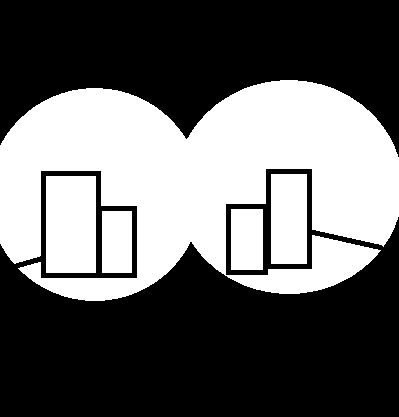
\includegraphics[width=0.8\linewidth]{graphics/tunnelvision.png}
		\caption{Tunnel Vision}	
		\label{ref:subref_a}
	\end{subfigure}%
	\begin{subfigure}{.5\textwidth}
		\centering
		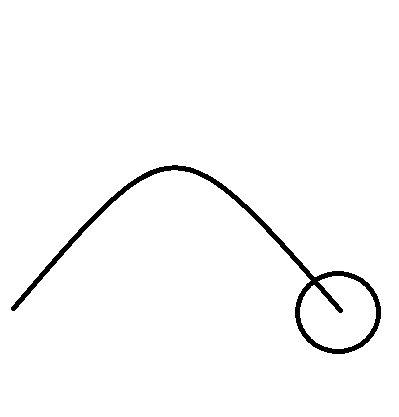
\includegraphics[width=0.8\linewidth]{graphics/teleportmove.png}
		\caption{Teleport Move}
		\label{ref:subref_b}
	\end{subfigure}%

\caption{Różny rodzaj poruszania się w programie}
\label{ref:ref}
\end{figure}
}
\subsection{Cześć Galerii Programu}
{\color{blue}
W tej części można poczytać i dowiedzieć się trochę o danym modelu. Swoim wyglądem przypomina to galerię obrazów, gdzie osoba podchodzi do danej ciekawostki i może ją przeczytać.
}
\subsection{Część pokazowa modeli programu programu}
{\color{blue}
Ta część galerii ma pokazać użytkownikowi programu w jaki sposób wygląda dany model w działaniu. Modele obsługuję się za pomocą kontrolerów ruchowych. W zależności od modelu interakcja wygląda trochę inaczej, szczegółowo każda zostanie omówiona w sekcji dotyczącej danego modelu. 
}
\section{Warstwa Programistyczna}

\subsection{Unreal Engine 4}
{\color{red}
Program był pisany w silniku Unreal Engine 4, z powodu że korzystam z tego silnika na codzień w swojej pracy. Sam silnik wspiera też bez większym problemów gogle VR, dzięki pluginowi stworzonemu przez twórców silnika. UE4 jest silnikiem wszechstronnym, czyli nie musi byc wykorzystywany tylko do tworzenia gier. Sam silnik jest dość popularny wśród ludzi co oznacza, że w  i nie tylko można znaleźć ogrom materiałów do pomocy przy projekcie. UE4 posiada wbudowany język skryptowy zwany BluePrint, opiera się głównie bloczkach które łączą się miedzy sobą. Głównym celem BP jest chęć zdobycia widowni wśród ludzi którzy na codzień nie programują i wolą patrzeć na coś milszego dla oka. Nody są podobne do tych wykorzystywanych w blenderze. Projekt w UE4 nie musi się opierać tylko na nodach, można też większość rzeczy pisać w C++.
\begin{figure}[H]%
\centering
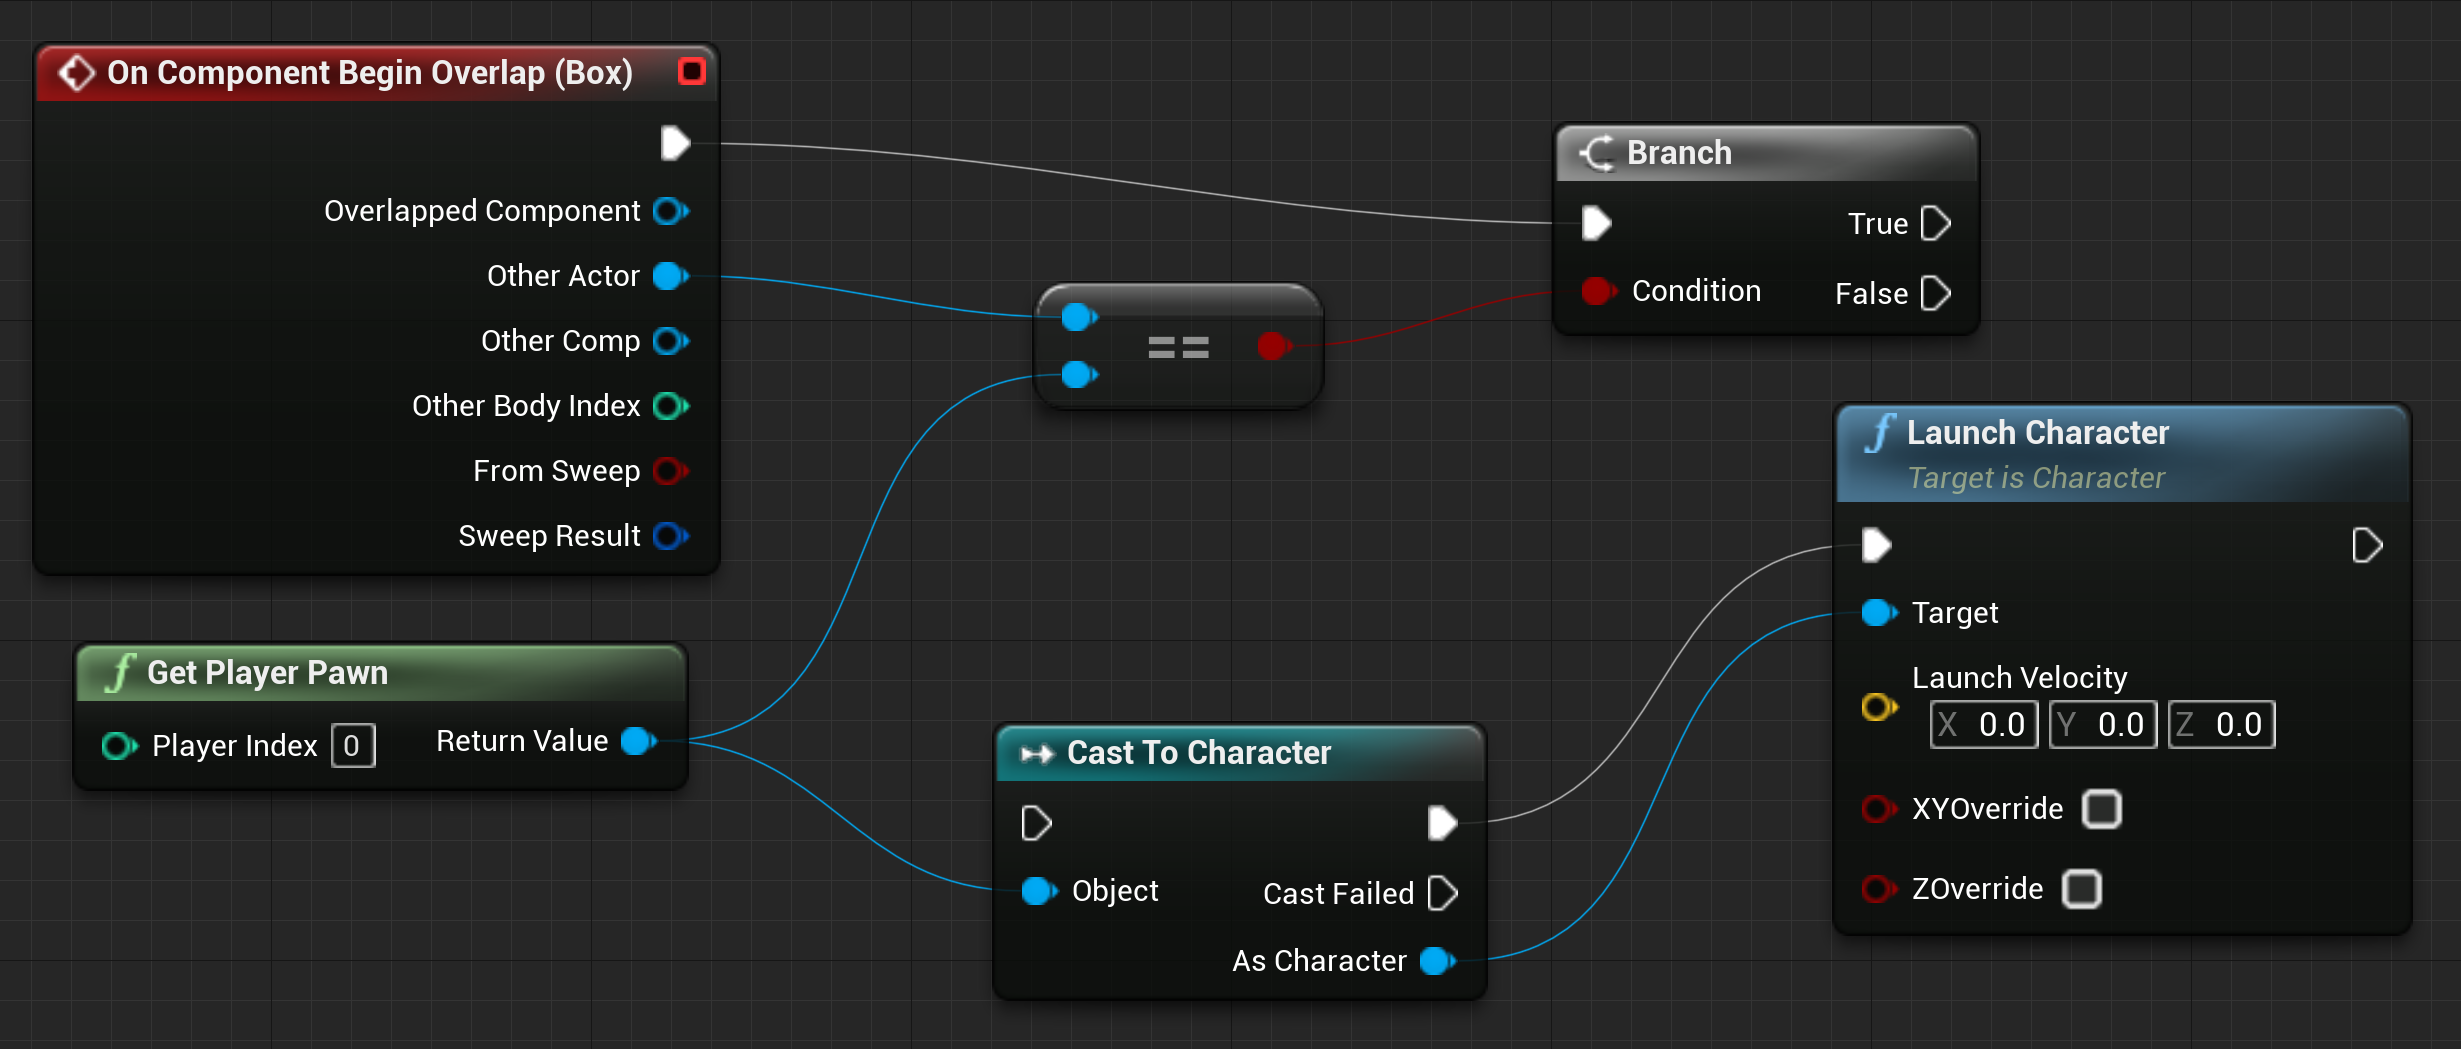
\includegraphics[width=0.8\columnwidth]{graphics/BPExample.png}
\caption{Przykładowy BluePrint w UE4
\label{BPExample}}%
%
\qquad
\end{figure}  

 Sam w silnik pozwala też na tworzenie poziomów w prosty i intuicyjny sposób, poprzez przeciąganie interesującego nas obiektu bezpośrednio na ekran a następnie, na jego obracanie czy nachylenie. W edytorze możemy też uruchomić interesujący na poziom i zobaczyć czy wszystko działa tak jak należy. Możemy też edytować materiał dla meshy na poziomię w podobny sposób jak tworzymy klasy aktorów, czyli poprzez nody. 
}
\subsection{Język C++}
{\color{red}
 UE4 pozwala też pisać klasy i funkcję w języku C++, a nie tylko w BP. Pisanie rzeczy C++ w UE4 nie różni się wiele od pisania w czystym C++, zaleca się oczywiście pisania rzeczy odwołujących się do biblioteki unrelea, co nie znaczy, że nie można niektóre pisać czysto w C++. Można oczywiście daną zmienną w klasie trzymać tylko w kodzie źródłowym, jeśli chcemy się odwołać do edytora UE4 i tam też coś robić musimy użyć specyfikator UPROPERTY przed zmienną i UFUNCTION przed funckja. Specyfikatory mają też dostępne opcję dzięki którym możemy np. edytować daną zmienna w edytorze lub podczas działania aplikacji. Najważniejszymi funckjami które dziedziczymi po klasach z biblioteki UE4 to Begin Play, Tick i EndPlay. BeginPlay uruchamia się kiedy dany aktor zostaję wywołany w czasię gry podsczas spawnu. Tick jest wywowyłany w każdym ticku życia aktora na poziomię. EndPlay jest wywoływany kiedy aktor kończy swój żywot. Danego aktora możemy zrobić czysto w C++ i tak samo go spawnować na levelu, ale lepiej jest stworzyć klasę dziedziczącą po nim w edytorze, staję się wtedy ona klasą BP którą możemy rozbudować o nowę funckje. Jeśli w klasię C++ stworzymy odwołonie do actor componenta, specjalna fuckcje (rozpisać co to), w klasię bp będzie widoczna jako odziedzicona po klasię C++.

\begin{figure}[H]%
\centering
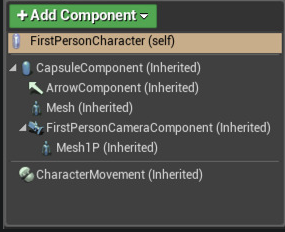
\includegraphics[width=0.8\columnwidth]{graphics/CppInherited.png}
\caption{W nawiasie informacja, że odziedziczone z po klasie bazowej
\label{CppInherited}}%
%
\qquad
\end{figure}   
 
  C++ pod względem działania funkcji jest szybszy od funkcji BP, więc z doświadczenia zalecam pisania głównie w nim i dopiero w mniejszym stopniu tworzyć jakieś małe funkcje pomocnicze w BP.
  }

\subsection{Oculus Quest}

{\color{red}
 Gogle VR z których korzystam to Oculus Quest 1. Aby komunikować się z nimy korzystam z obrogramowania storzonym przez firmę Oculus, dzięki niemu mogę obsługiwać gogle na komputerzę przez sieć WiFi, a nie przez podłączenie gogli po kablu do komputera. Gogle te nie potrzebują do pracy komputera, poniewasz są w pełni autonomiczne, cała technologia skrywa się w samych goglach, dzięki czemu nie są potrzebne stacje bazowe. Aby tworzyć programy na goglach nie trzeba się specjalnie męczyć, trzeba oczywiście stowrzyć sterowania i komunikajcę ze światem wirtualnym przystosowanym specjalnie pod sterowanie ruchowe, oraz dostosawnie grafiki, aby ilośc FPS nie spadała poniżej 72 i utrzymywała je stale na tej wartości, dzięki temu nie ma większych problemów z chorobą symulatorową dla większości osób
}

\section{Jakie modele się znajdują}

\subsection{Wahadło Podwójne}

\begin{figure}[H]%
\centering
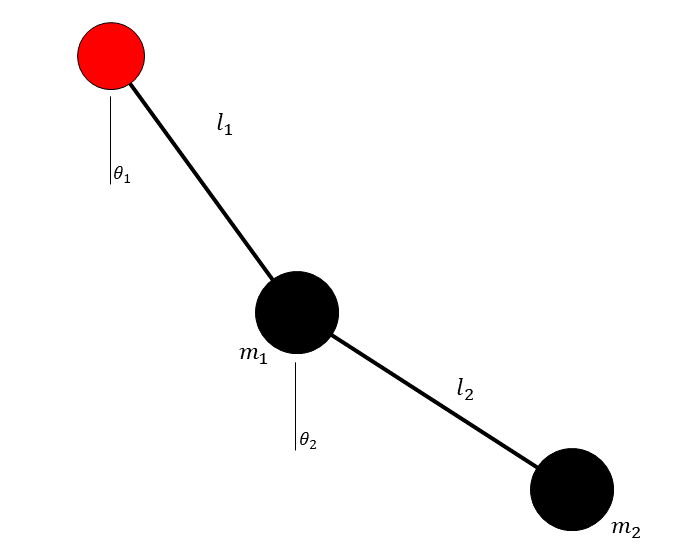
\includegraphics[width=0.5\columnwidth]{graphics/DoublePendulum.png}
\caption{$\theta$ 1-2 kąty swobodne, m1 m2 masy obiektów, l1 l2 długości pręta
\label{BPExample}}%
%
\qquad
\end{figure}  


Pierwszy model który umieściłem jest model wahadła podwójnego. Wahadło podwójne, jest wahadłem które ma przymocowane drugie wahadło na jego końcu. \cite{double_pendulum} W wahadle tym punkty masy są na końcu każdego pręta o danej długości. Wahadła obracają się swobodnie w płaszczyźnie pionowej. Energię potencjalną wahadła podwójnego oblicza się jako odniesienie uniesionego wahadła do stanu zerowej energii potencjalnej w położeniu równowagi, Dlatego równanie ma następującą postać: 

\begin{equation} 
V=m_1gl_1(1-\cos\theta_1)+m_2g[l_1(1-\cos\theta_1)+l_2(1-\cos\theta_2)]
\end{equation}

W celu sformułowania równania energii kinetycznej wykorzystamy wyprowadzenie współrzędnych x i y układu, które przedstawiono poniżej:

\begin{equation}
\begin{split} 
x_2=l_1\sin\theta_1+l_2\sin\theta_2\\
y_2=l_1\cos\theta_1-l_2\cos\theta_2
\end{split}
\end{equation}

Po wyprowadzeniu i zsumowaniu wyrażeń możemy określić ostateczną postać energii kinetycznej:

\begin{equation}
\begin{split} 
K=\frac{1}{2}m_1l_1^2\dot{\theta_1^2}+\frac{1}{2}m_2l_1^2\dot{\theta_1^2}+\frac{1}{2}m_2l_2^2\dot{\theta_2^2}+m_2l_1l_2\cos(\theta_1-\theta_2)\dot{\theta_1}\dot{\theta_2}
\end{split}
\end{equation}


Najprostsze równanie Lagrange ma postać:

\begin{equation}
\begin{split} 
\frac{d}{dt}(\frac{\partial L}{d\dot{\theta_i}})-(\frac{\partial L}{d\theta_i})=0
\end{split}
\end{equation}

Korzystając z równań Lagrange i dokonując odpowiednich podstawień, możemy sformułować sprzężone równanie ruchu dla podanego układu:

\begin{equation}
\begin{split} 
\ddot{\theta_1}=-\frac{l_2}{\mu l_1} \ddot{\theta_2}\cos(\theta_1-\theta_2)-\frac{l_2}{\mu l_1}\dot{\theta_2^2} sin(\theta_1-\theta_2)-\frac{g}{l_1}\sin\theta_1\\
\ddot{\theta_2}=-\frac{l_1}{l_2} \ddot{\theta_1}\cos(\theta_1-\theta_2)-\frac{l_1}{l_2}\dot{\theta_1^2} sin(\theta_1-\theta_2)-\frac{g}{l_2}\sin\theta_2\\
\end{split}
\end{equation}

gdzie:
\begin{equation}
\begin{split} 
\mu=1+(m_1+m_2)
\end{split}
\end{equation}

Aby zdekomponować pojęcia przyspieszenia kątowego, podstawiamy je, wstawiając drugie równanie do pierwszego i odwrotnie, otrzymujemy: 

\begin{equation}
\begin{split} 
\ddot{\theta_1}=\frac{g(\sin\theta_2\cos(\theta_1-\theta_2)-\mu\sin\theta_1)
-(l_2\dot{\theta_2^2}+l_1\dot{\theta_1^2}\cos(\theta_1-\theta_2))\sin(\theta_1-\theta_2)}{l_1(\mu-\cos^2(\theta_1-\theta_2))}
\\
\ddot{\theta_1}=\frac{g\mu(\sin\theta_1\cos(\theta_1-\theta_2)-\sin\theta_2)
-(\mu l_1\dot{\theta_1^2}+l_2\dot{\theta_2^2}\cos(\theta_1-\theta_2))\sin(\theta_1-\theta_2)}
{l_2(\mu-\cos^2(\theta_1-\theta_2))}
\\
\end{split}
\end{equation}


 nowych zmienny w1 i w2 pozwala na sformułowanie czterech równań co ułatwia rozwiązanie numeryczne:
 
 
\begin{equation}
\begin{split} 
\dot{\theta_1}=\omega_1\\\\
\omega_1=\frac{g(\sin\theta_2\cos(\theta_1-\theta_2)-\mu\sin\theta_1)
-(l_2\dot{\theta_2^2}+l_1\dot{\theta_1^2}\cos(\theta_1-\theta_2))\sin(\theta_1-\theta_2)}{l_1(\mu-\cos^2(\theta_1-\theta_2))}
\\
\dot{\theta_1}=\omega_2\\\\
\omega_2=\frac{g\mu(\sin\theta_1\cos(\theta_1-\theta_2)-\sin\theta_2)
-(\mu l_1\dot{\theta_1^2}+l_2\dot{\theta_2^2}\cos(\theta_1-\theta_2))\sin(\theta_1-\theta_2)}
{l_2(\mu-\cos^2(\theta_1-\theta_2))}
\\
\end{split}
\label{computeAnglesEuler}
\end{equation}


\subsubsection{Wahadło podwójne - kod}


W C++ kod wahadła składa się z trzech klas: Pendulum, PendulumSpawn, PendulumControl

W klasie Pendulum, wahadło podwójne jest stworzone z Spline, na podstawie danych pozycji X i Y jest aktualizowany co klatkę. Na początku wahadło podwójne jest tworzone na podstawie otrzymanych wartości w metodzie SetParameters

\begin{lstlisting}
void SetParameters(double _theta0, double _length0, double _mass0, double _theta1, double _length1, double _mass1);
\end{lstlisting}

Na podstawie tych równań (\ref{computeAnglesEuler}) stworzyłem metodę która obliczą theta wahadeł do obliczenia ich obecnej pozycji w programie:

\begin{lstlisting}
void APendulum::computeAnglesEuler(float dt)
{
	double u = 1 + mass0 + mass1;
	theta0bis =
		(g * (sin(theta1) * cos(theta0 - theta1) - u * sin(theta0))
			- (length1 * pow(theta1prim, 2) + length0 * pow(theta0prim, 2) * cos(theta0 - theta1)) * sin(theta0 - theta1))
		/ (length0 * (u - pow(cos(theta0 - theta1), 2)));
	theta1bis =
		(g * u * (sin(theta0) * cos(theta0 - theta1) - sin(theta1)) + (u * length0 * pow(theta0prim, 2)
			+ length1 * pow(theta1prim, 2) * cos(theta0 - theta1)) * sin(theta0 - theta1))
		/ (length1 * (u - pow(cos(theta0 - theta1), 2)));


	theta0prim = theta0prim + theta0bis * dt;
	theta1prim = theta1prim + theta1bis * dt;

	theta0 = theta0 + theta0prim * dt;
	theta1 = theta1 + theta1prim * dt;
}
\end{lstlisting}


Następnie wyliczone wartości są wykorzystywane do obliczania pozycji wahadła w metodzie computePosition i aktualizowana jest w nim pozycja Spline:

\begin{lstlisting}
void APendulum::computePosition()
{
	x0 = px + length0 * FMath::Sin(theta0);
	y0 = py + length0 * FMath::Cos(theta0);

	x1 = x0 + length1 * FMath::Sin(theta1);
	y1 = y0 + length1 * FMath::Cos(theta1);
	auto Frector = GetActorLocation();
	FVector StarPos1 = { Frector.X, px,py, };
	FVector EndPos1 = { Frector.X, x0, y0, };

	//FVector StarPos2 = { x0, y0,Frector.Z+150 };
	FVector EndPos2 = { Frector.X,x1, y1, };

	TArray<FVector> Path;
	Path.Add(StarPos1);
	Path.Add(EndPos1);
	Path.Add(EndPos2);

	FirstColumn->ClearSplinePoints(false);
	int32 index = 0;
	for (auto& Point : Path)
	{
		FVector LocalPosition = FirstColumn->GetComponentTransform().InverseTransformPosition(Point);
		FirstColumn->AddPoint(FSplinePoint(index, LocalPosition, ESplinePointType::Constant), false);
		index++;
	}

	FirstColumn->UpdateSpline();

	int32 SegmentNum = Path.Num() - 1;
	for (int32 i = 0; i < SegmentNum; ++i)
	{
		if (ColumnsPathMeshPool.Num() <= i)
		{
			USplineMeshComponent* SplineMesh = NewObject<USplineMeshComponent>(this);
			SplineMesh->SetMobility(EComponentMobility::Movable);
			SplineMesh->AttachToComponent(FirstColumn, FAttachmentTransformRules::KeepRelativeTransform);
			SplineMesh->SetStaticMesh(FirstColumnArchMesh);
			SplineMesh->SetMaterial(0, FirstColumnArchMaterial);
			SplineMesh->RegisterComponent();

			ColumnsPathMeshPool.Add(SplineMesh);
		}

		USplineMeshComponent* SplineMesh = ColumnsPathMeshPool[i];
		SplineMesh->SetVisibility(true);

		FVector StarPos, StartTangent, EndPos, EndTangent;
		FVector Tangent = { 0,0,0 };
		FirstColumn->GetLocalLocationAndTangentAtSplinePoint(i, StarPos, StartTangent);
		FirstColumn->GetLocalLocationAndTangentAtSplinePoint(i + 1, EndPos, EndTangent);
		SplineMesh->SetStartAndEnd(StarPos, Tangent, EndPos, Tangent);

	}

}
\end{lstlisting}

Klasa PendulumSpawn jest odpowiedzialna za dodawanie i usuwanie wahadeł oraz jest odpowiedzialna za uruchamianie i resetowanie wszystkich aktualnych wahadeł na scenie
Klasa ma też wskaźnik na klasę PendulumControl która ta jest odpowiedzialna za stworzenie UI dzięki któremu użytkownik może obsługiwać wahadła.

\subsubsection{Wahadło podwójne - UE4}
Na podstawie powyższych klas zostały stworzone klasy BluePrintowe które można potem umieścić w na poziomie w programie. BP\_Pendulum ma tylko informację o tym jak Spline ma wyglądać w świecie gry:

\begin{figure}[H]%
\centering
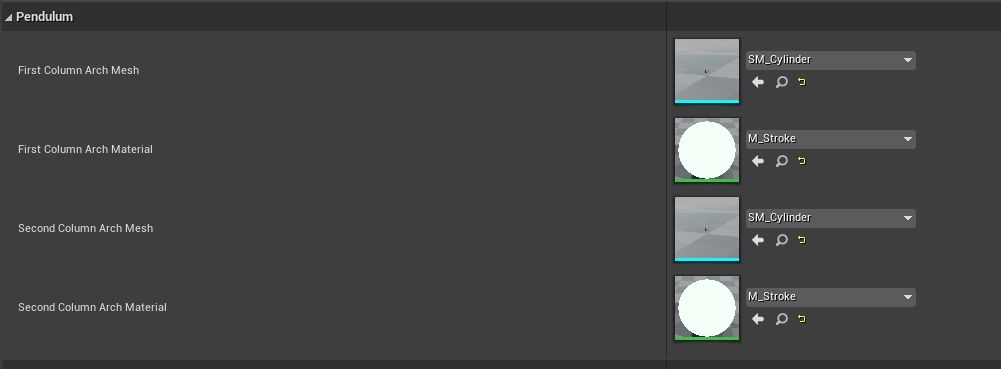
\includegraphics[width=0.7\columnwidth]{graphics/PendulumBP.png}
\caption{Ustawiony mesh i tekstura dla wahadła 
\label{BPExample}}%
%
\qquad
\end{figure}  

BP\_PendulumSpawn jest aktorem który zostaje umieszczony na poziomie, trzeba tylko ustawić w nim informację o wahadle które chcemy stworzyć na poziomie oraz jaki widget chcemy umieścić by można za jego pomocą sterować wahadłami.

\begin{figure}[H]%
\centering
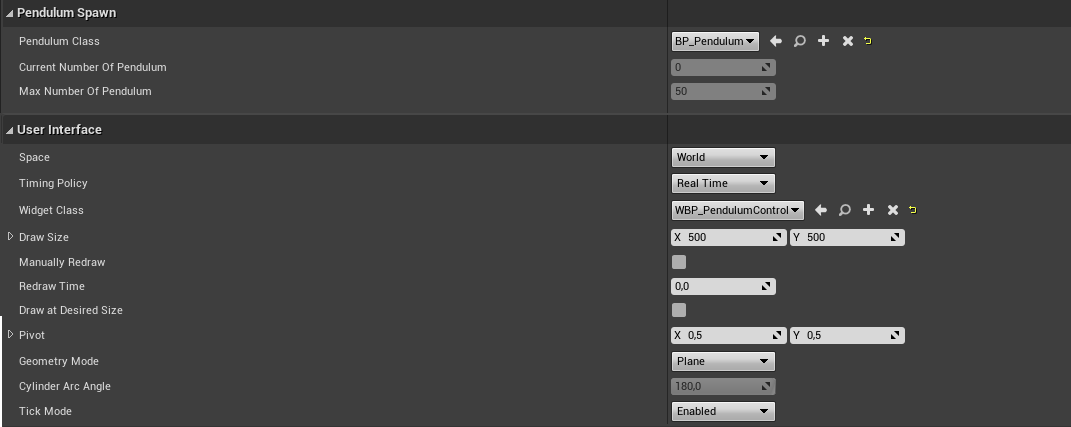
\includegraphics[width=0.7\columnwidth]{graphics/PendulumSpawnerBP.png}
\caption{Ustawione wahadło do stworzenia i widget 
\label{BPExample}}%
%
\qquad
\end{figure}  

Klasa WBP\_PendulumControl jest odpowiedzialna kontakt miedzy użytkownikiem a programem, klasa ta jest widgetem dzięki któremu poprzez najechanie kontrolerem ruchowym na odpowiednie opcje możemy dodać lub usunąć wahadło oraz włączyć lub zresetować wszystkie wahadła podpięte pod dany spawner 

\begin{figure}[H]%
\centering
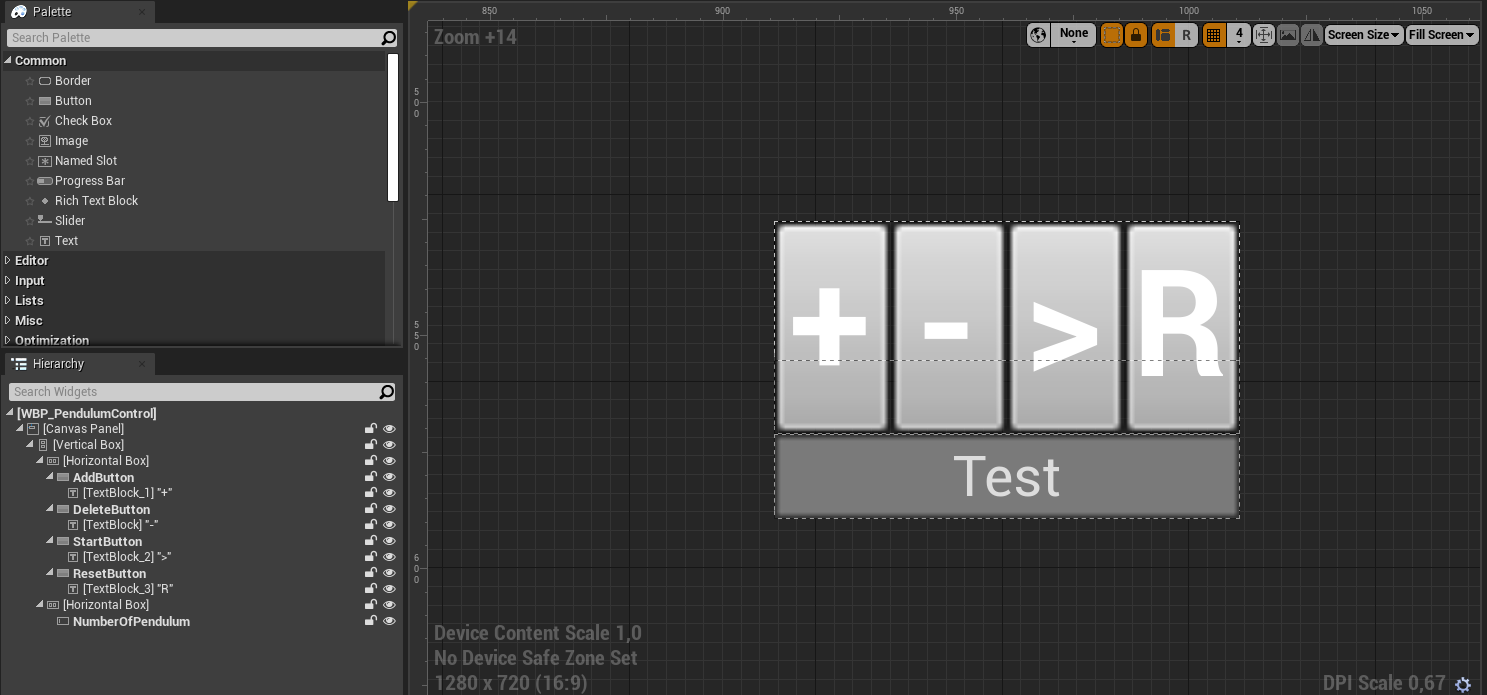
\includegraphics[width=0.7\columnwidth]{graphics/PendulumControlBP.png}
\caption{Wygląd widgetu w programie
\label{BPExample}}%
%
\qquad
\end{figure}  

\subsubsection{Wahadło podwójne - Wygląd w programie}
W programie wahadło wygląda następująco:


\begin{figure}[H]%
	\centering
	\begin{subfigure}{.5\textwidth}
		\centering
		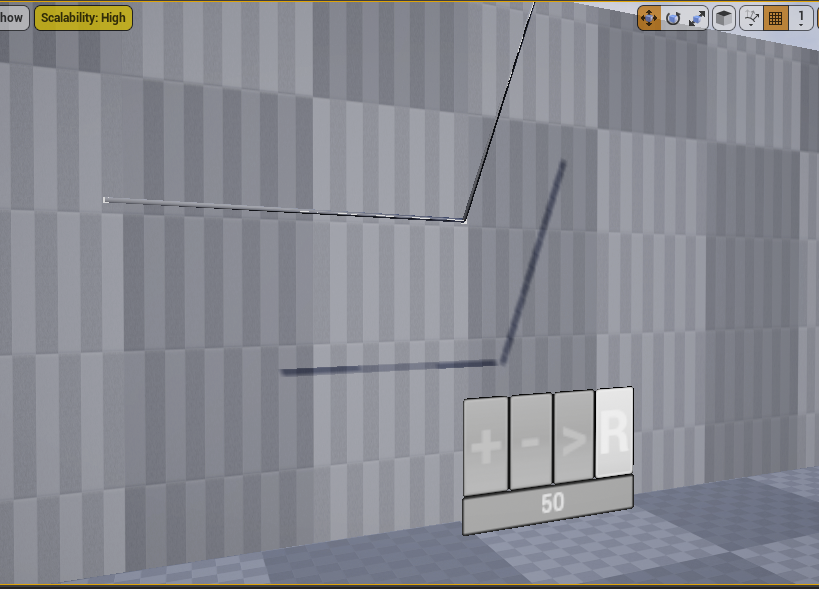
\includegraphics[width=0.8\linewidth]{graphics/PendulumInUE_1.png}
		\caption{Wahadła na początku symulacji}	
		\label{ref:subref_a}
	\end{subfigure}%
	\begin{subfigure}{.5\textwidth}
		\centering
		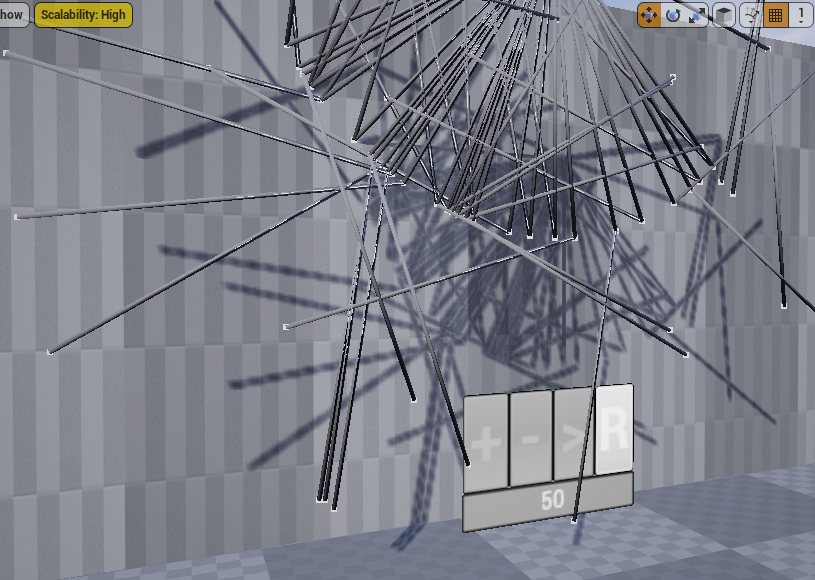
\includegraphics[width=0.8\linewidth]{graphics/PendulumInUE_2.png}
		\caption{Wahadła na końcu symulacji}
		\label{ref:subref_b}
	\end{subfigure}%
	

\caption{Działanie programu}
\label{ref:ref}
\end{figure}

\subsection{Gra w życie}

Gra w życie została wymyślona w 1970 przez Johna Conwaya zainpirowany pracami Stanisława Ulmana. Gra w życie jest automatem komórkowym, czyli jest to system składający się z pojedynczych komórek działający według określonych reguł.\cite{game_of_life} W przypadku gry w życie, dana komórka, ma ośmiu sąsiadów przylegających do niej bokami i rogami w jednej chwili może być żywa lub martwa, a to czy żyje określają 4 zasady:\\
1.Żywa komórka, która ma mniej niż dwóch sąsiadów, w kolejnym kroku umiera. \\
2.Żywa komórka, która ma więcej niż trzech sąsiadów, umiera.\\
3.Żywa komórka, która ma dwóch lub trzech sąsiadów – przeżywa.\\
4.Martwa komórka, która ma trzech żywych sąsiadów – ożywa.\\

Gra w życię nie jest do końca grą, rola "gracza" ogranicza się ustawienia stanu początkowego planszy, poprzez ożywianie lub uśmiercanie danej komórki.\cite{game_of_life_wiki}


\subsubsection{Gra w życie - kod}

W C++ kod gry w życie składa się z trzech klas: CellActor, GridActor, GameOfLifeControl

CellActor jest klasą w której znajdują się informację o jednej komórce znajdującej w siatce. Sama w sobie ma informację o swoim położeniu X i Y na siatce 2D, o swoim obecnym stanie życia oraz o stanie życia w następnej klatce trwania programu. 
Kiedy użytkownik najedzie na daną komórkę i kliknie spust w metodzie Clicked zmieni stan początkowy komórki z martwą na żywą i vice versa.
\begin{lstlisting}
void ACellActor::Clicked()
{
		if (Alive) {
			StaticMeshComponent->SetMaterial(0, BeginCursorOverMaterial);
			Alive = false;
		}
		else {
			StaticMeshComponent->SetMaterial(0, ClickedMaterial);
			Alive = true;
		}
}
\end{lstlisting}

W metodzie Update która jest wykorzystywana przez GridActora podbnie jak w metodzie Clicked na podstawie zmiennej AliveNext używia, pozostawia przy życiu lub uśmierca daną komórkę

\begin{lstlisting} 
void ACellActor::Update()
{
	if (AliveNext) {
		StaticMeshComponent->SetMaterial(0, ClickedMaterial);
		Alive = true;
		SetActorHiddenInGame(false);
	}
	else {
		SetActorHiddenInGame(true);
		StaticMeshComponent->SetMaterial(0, EndCursorOverMaterial);
		Alive = false;
	}
}
\end{lstlisting}


Klasa ma też Gettery i Settery odpowiedzialne, za branie informacji o obebcnym stanie komórki jak i o jej stanie w następnej klatce
\begin{lstlisting}[frame=single]  % Start your code-block
	bool GetAlive() const {
		return Alive;
	}
	void SetAlive(const bool IsAlive) {
		this->Alive = IsAlive;
	}

	bool GetAliveNext() const {
		return AliveNext;
	}
	void SetAliveNext(const bool IsAliveNext)
	{
		this->AliveNext = IsAliveNext;
	}

\end{lstlisting}

Klasa GridActor jest odpowiedzialna za tworzenie siatki 2D z klasy CellActor o podanej wielkości. W samej klasie dzieją się też wszystkie obliczenia związane z działaniem gry w życie od obliczania obecnie żyjących sąsiadów danej komórki w metodzie CountAliveNeighbors(const int i, const int j)

\begin{lstlisting}
int AGridActor::CountAliveNeighbors(const int i, const int j) {
	int NumAliveNeighbors = 0;
	for (int k = -1; k <= 1; k++) {
		for (int l = -1; l <= 1; l++) {
			if (!(l == 0 && k == 0)) {
				const int effective_i = i + k;
				const int effective_j = j + l;
				if ((effective_i >= 0 && effective_i < Height) && (effective_j >= 0 && effective_j < Width)) {
					if (CellActors[effective_j + effective_i * Width]->GetAlive()) {
						NumAliveNeighbors++;
					}
				}
			}
		}
	}
	return NumAliveNeighbors;
}
\end{lstlisting}

Następnie na podstawie obecnie żyjących sąsiadów i reguł jakie zostały ustawione w metodzie UpdateAliveNext(const int Index, const int NumAliveNeighbors) ustawiamy czy dana komórka w następnej klatce będzie żywa lub martwa

\begin{lstlisting}
void AGridActor::UpdateAliveNext(const int Index, const int NumAliveNeighbors) {
	const bool IsAlive = CellActors[Index]->GetAlive();
	if (IsAlive && (NumAliveNeighbors < 2))
	{
		CellActors[Index]->SetAliveNext(false);
	}
	else if (IsAlive && ((NumAliveNeighbors == 2) || (NumAliveNeighbors == 3)))
	{
		CellActors[Index]->SetAliveNext(true);
	}
	else if (IsAlive && (NumAliveNeighbors > 3))
	{
		CellActors[Index]->SetAliveNext(false);
	}
	else if (!IsAlive && (NumAliveNeighbors == 3))
	{
		CellActors[Index]->SetAliveNext(true);
	}
	else {
		CellActors[Index]->SetAliveNext(CellActors[Index]->GetAlive());
	}
}
\end{lstlisting}

Stworzona została jeszcze wersja 3D GridActora którego jedyną różnicą jest to, że na została dodana też głębokość.

Ostatnią klasą jest GameOfLifeControll która jest odpowiedzialna
za stworzenie UI dzięki któremu użytkownik może włączyć grę w życie, zmienać szybkość działania symulacji oraz resetowania jej do stanu początkowego.

\subsubsection{Gra w życie - UE4}

Na podstawie powyższych klas zostały stworzone klasy BluePrintowe które można potem umieścić w na poziomie w programie. W BP\_CellActor ustawiamy jak dana komórka ma wyglądać w świecie gry i jak się zachować kiedy najedziemy na nią kontrolerem ruchowym:

\begin{figure}[H]%
	\centering
	\begin{subfigure}{.45\textwidth}
		\centering
		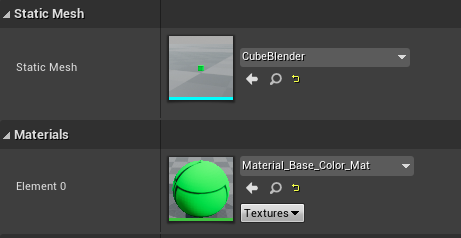
\includegraphics[width=0.8\linewidth]{graphics/CellActorInUE_1.png}
		\caption{Ustawiony mesh w programie dla komórki}	
		\label{ref:subref_a}
	\end{subfigure}%
	\begin{subfigure}{.45\textwidth}
		\centering
		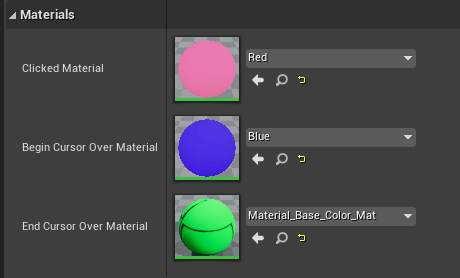
\includegraphics[width=0.8\linewidth]{graphics/CellActorInUE_2.png}
		\caption{Ustawiony wygląd w programie podczas akcji}
		\label{ref:subref_b}
	\end{subfigure}%
	

\caption{Ustawienia dla CellActora w UE4}
\label{ref:ref}
\end{figure}

BP\_GridActor2D jest klasą BluePrint która znajdzie się na poziomie gry. W klasie ustawiamy na jaką szerokość i wysokość ma zostać stworzona siatka składająca się z BP\_CellActor oraz dodajemy widget, dzięki któremu możemy sterować symulacją:

\begin{figure}[H]%
\centering
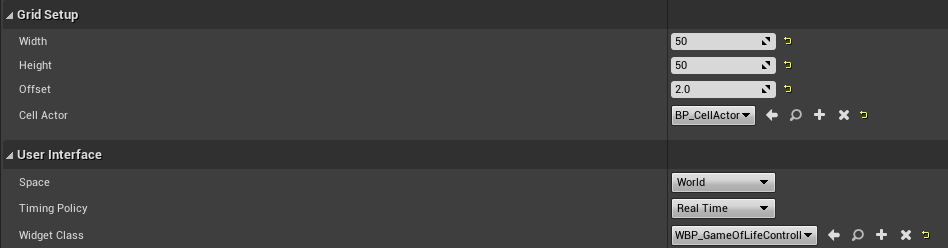
\includegraphics[width=0.7\columnwidth]{graphics/GridActor2DInUE_1.png}
\caption{Ustawienia BP\_GridActor2D 
\label{BPExample}}%
%
\qquad
\end{figure}  

Na podobnej zasadzie działa BP\_GridActor3D w którym dochodzi jeszcze głębokość na którą możemy ustawić siatkę.\\

Klasa WBP\_GameOfLifeControll jest odpowiedzialna kontakt miedzy użytkownikiem a programem, klasa ta jest widgetem dzięki któremu poprzez najechanie kontrolerem ruchowym na odpowiednie opcje możemy włączyć symulację, przyśpieszyć lub ją spowolnić oraz ją zresetować do stanu początkowego:

\begin{figure}[H]%
\centering
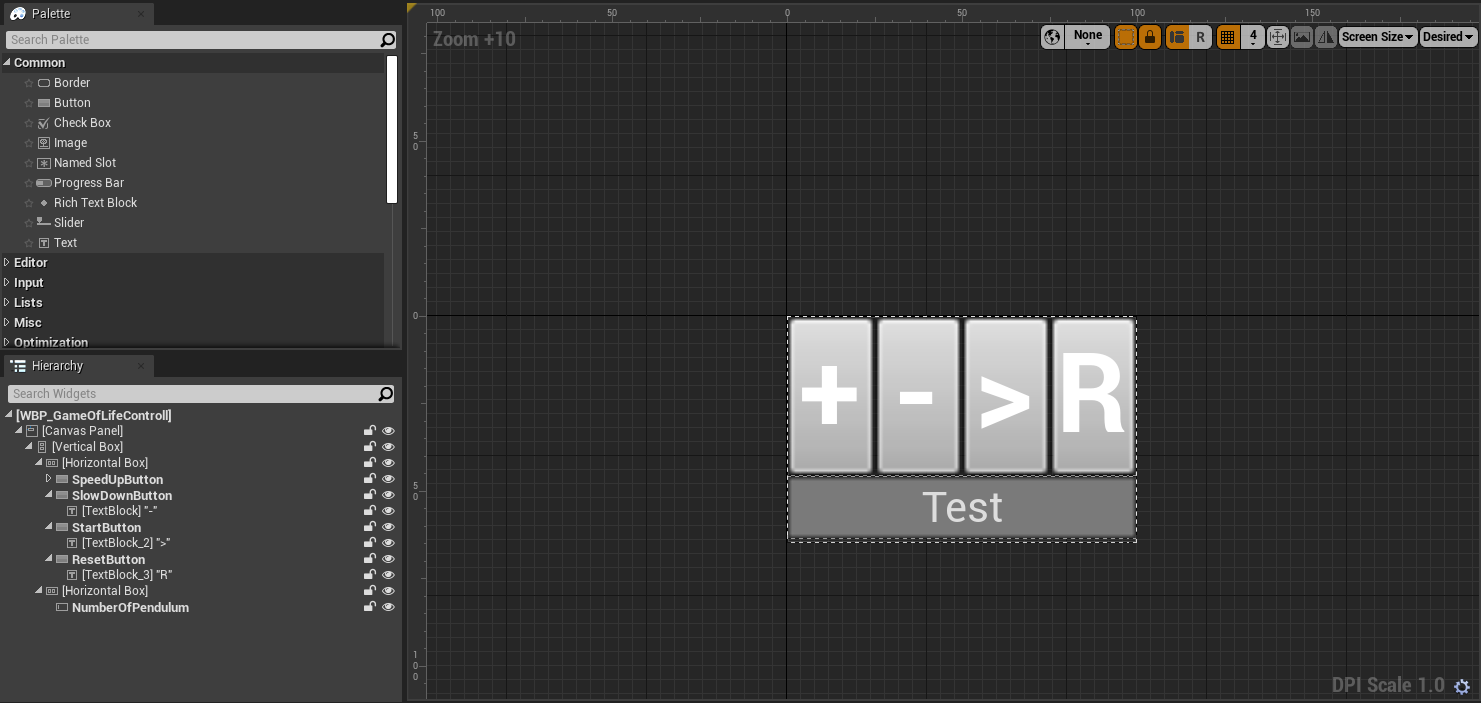
\includegraphics[width=0.7\columnwidth]{graphics/GameOfLifeControllInUE_1.png}
\caption{Wygląd widgetu w programie
\label{BPExample}}%
%
\qquad
\end{figure}  

\subsubsection{Gra w życie - Wygląd w programie}
W programie Gra w życie wygląda następująco:


\begin{figure}[H]%
	\centering
	\begin{subfigure}{.5\textwidth}
		\centering
		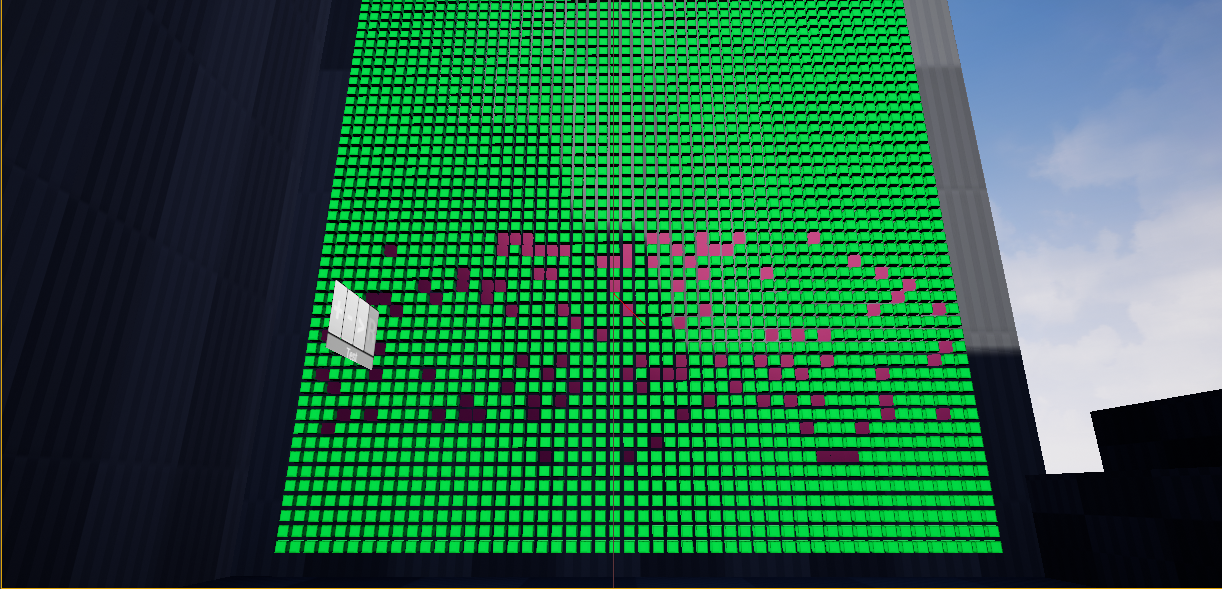
\includegraphics[width=0.8\linewidth]{graphics/GOLInUE_1.png}
		\caption{Gra w życie podczas ustawia stanu początkowego}	
		\label{ref:subref_a}
	\end{subfigure}%
	\begin{subfigure}{.5\textwidth}
		\centering
		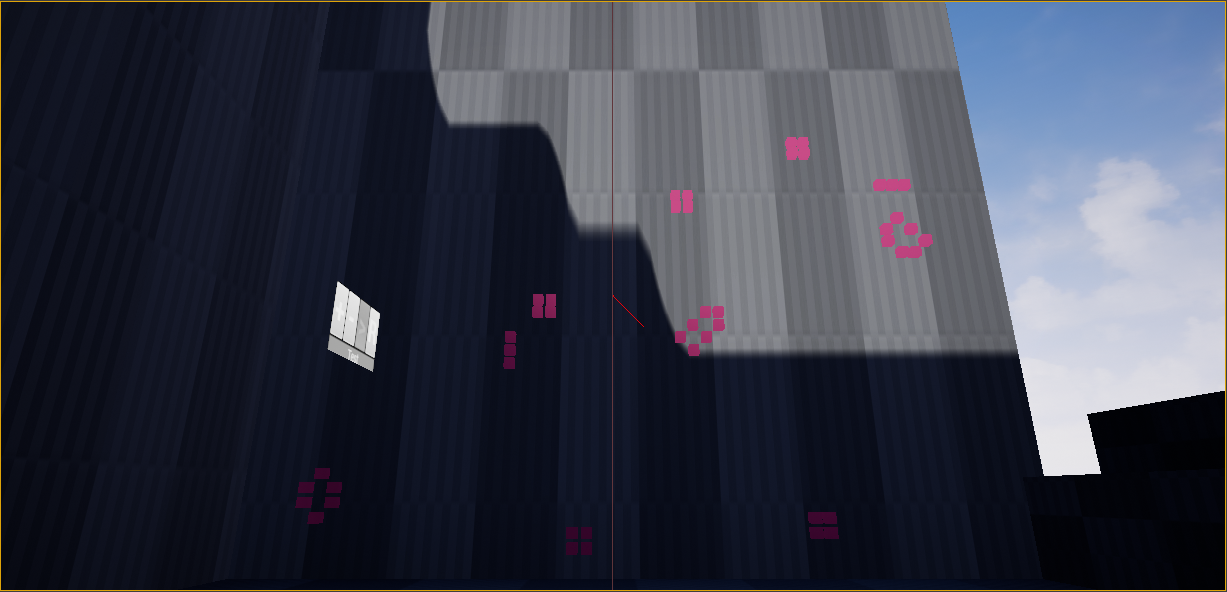
\includegraphics[width=0.8\linewidth]{graphics/GOLInUE_2.png}
		\caption{Gra w życie w trakcie trwania symulacji}
		\label{ref:subref_b}
	\end{subfigure}%
	

\caption{Działanie programu}
\label{ref:ref}
\end{figure}

\subsection{Efekt Motyla}

"Dowolny układ fizyczny, który zachowuje się nieokresowo, jest nieprzewidywalny." Są to słowa Edwarda Lorenza, meteorologa który jako pierwszy odkrył, że nie można zrobić dobrej prognozy pogody na dłużej niż kilka dni do przodu. W 1960 roku pracował on nad programem komputerowym który miał prognozować pogodę, na podstawie zbioru równań określających zależności między prędkością wiatru, temperaturą, ciśnieniem i wilgotnością. Gdy Lorenz testował swój program po wprowadzeniu danych i po wydrukowaniu wyniku w formie wykresu. Rozkład maksimów i minimów na wykresie wyglądał tak, jak się tego spodziewał Edward. Postanowił jednak ponownie zbadać wyniki, dlatego uruchomił program ponownie, wprowadzając jak myślał takie same wyniki. Okazało się jednak, że wyniki wyszły na odwrót. Po sprawdzeniu danych zauważył, że podał je w postaci przybliżonej z mniejszą liczbą cyfr po przecinku. Było to dla niego tak ciekawe, że spróbował to samo z innymi zbiorami danych i zaobserwował identyczne zjawisko. Lorenz w ten sposób odkrył "efekt motyla", gdzie dla pewnych układów deterministycznych nawet minimalne zmiany wartości danych początkowych zostają bardzo szybko wzmocnione i powodują ogromne zmiany w ewolucji układu\cite{burze_motyle}.

\begin{figure}[H]%
\centering
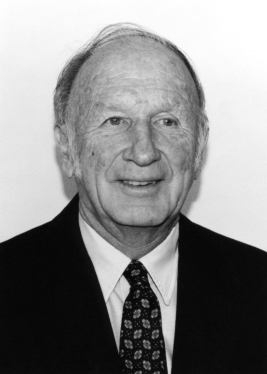
\includegraphics[width=0.4\columnwidth]{graphics/Edward_lorenz.jpg}
\caption{Edward Norton Lorenz 1917-2008 
\label{BPExample}}%
%
\qquad
\end{figure} 

Obecnie układ Lorenza jest bardziej znany jako układ 3 nieliniowych
równań różniczkowych:

\begin{equation}
\begin{split}
\dot{x}=\sigma(y-x)\\
\dot{y}=x(\rho-z)-y\\
\dot{z}=xy-\beta z\\
\end{split}
\end{equation}

gdzie:\\
sigma - stała Prandtla,\\
rho - stała Rayleigha,\\
beta - obszar obejmujący równania\\
sigma,rho,beta>0,\\
Jednakże zwykle podaje się:\\
sigma = 10, rho =8/3, beta jest zmienne.\\

\subsubsection{Efekt Motyla - kod}

Kod C++ składa się z dwóch klas ButterflyActor i ButterflySpawner.

W ButterflyActor najważnejszą metodą jest Tick(float DeltaTime) w której poprzez rozwązanie wczęśniej pokazanych równań różniczkowych po przecałkowaniu. Następnie odpowiednio ustawiamy te równania dla pozycji X, Y i Z danego aktora\cite{motyle_cpp}

\begin{lstlisting}
void AButterflyActor::Tick(float DeltaTime)
{
	Super::Tick(DeltaTime);
	DeltaTime = ButterflyChange;
	auto position = GetActorLocation();

	position.X = (position.X + sigma * (position.Y - position.X) * DeltaTime);
	position.Y = (position.Y + (-position.X * position.Z + rho * position.X - position.Y) * DeltaTime);
	position.Z = (position.Z + (position.X * position.Y - beta * position.Z) * DeltaTime);

	SetActorLocation(position);
}
\end{lstlisting}

Jedyną rolą ButterflySpawner jest utworzenie tyle ButterflyActor ile zostanie mu zadane na początku, z drobną zmianą odległości dla każdego kolejnego aktora.


\begin{lstlisting}
	for (size_t i = 0; i < numberOfButterfly; i++)
	{
		const FVector Loc(Origin.X + i * 15, Origin.Y, Origin.Z);
		AButterflyActor* const SpawnedActorRef = GetWorld()->SpawnActor<AButterflyActor>(ButterflyActor, Loc, GetActorRotation());
		ButterflyActors.Add(SpawnedActorRef);
	}
\end{lstlisting}

\subsubsection{Efekt Motyla - UE4}

Na podstawie powyższych klas zostały stworzone klasy BluePrintowe które można potem umieścić w na poziomie w programie. W BP\_ButterflyActor dla którego stworzyłem efekt cząsteczkowy który zostawia ścieżką jaką poruszał się dany aktor.

\begin{figure}[H]%
\centering
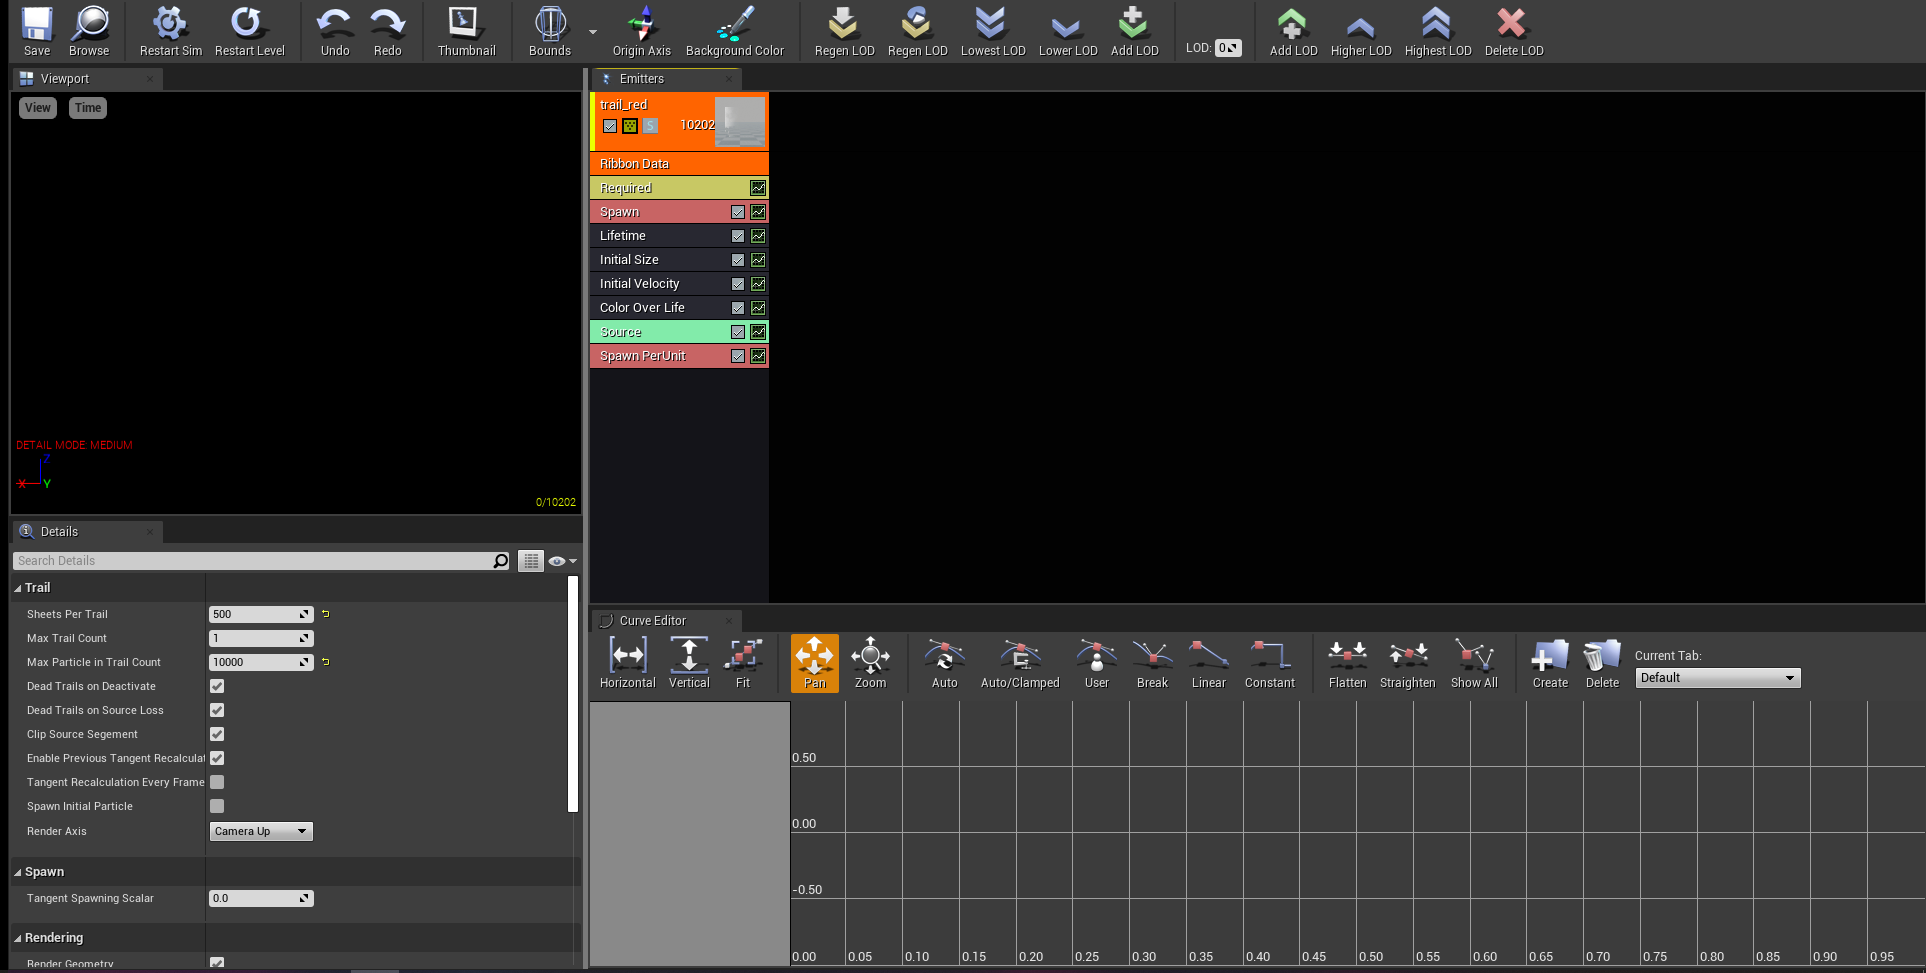
\includegraphics[width=0.7\columnwidth]{graphics/ButterflyParticleSystem.png}
\caption{Wygląd menu do tworzenia efektów cząsteczkowych w UE4 
\label{BPExample}}%
%
\qquad
\end{figure} 


W BP\_ButterflySpawner ustawiamy jakiego aktora chcemy ustawić na scenie, oraz ile motyli chcemy stworzyć.

\begin{figure}[H]%
\centering
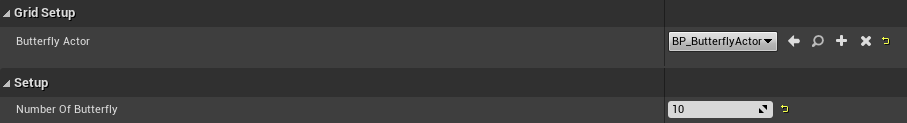
\includegraphics[width=0.7\columnwidth]{graphics/ButterflySpawner.png}
\caption{Wygląd menu do tworzenia efektów cząsteczkowych w UE4 
\label{BPExample}}%
%
\qquad
\end{figure} 



\subsubsection{Efekt Motyla - Wygląd w programie}
W programie Efekt Motyla wygląda następująco:

\begin{figure}[H]%
\centering
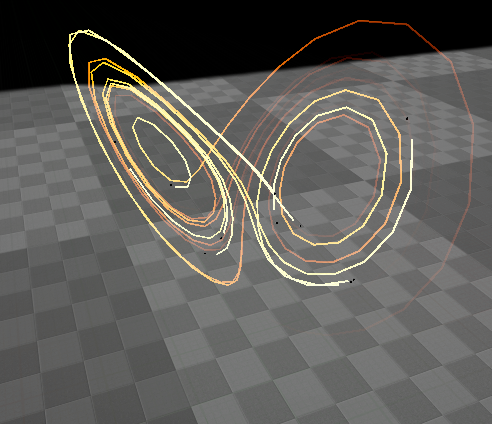
\includegraphics[width=0.7\columnwidth]{graphics/ButterflyInUE_1.png}
\caption{Wygląd widgetu w programie
\label{BPExample}}%
%
\qquad
\end{figure}  

\subsection{Model Agentowy}
\subsubsection{Model Agentowy - kod}
\subsection{Boids}
\subsubsection{Boids - kod}





\section{Realizacja projektu}

\section{Wnioski}


\newpage

\bibliographystyle{unsrt}
\bibliography{bibliografia}

{\color{blue} kolor blue: rozpisać}\\
{\color{red} kolor red: edytować i może dodać}\\
{\color{green} kolor green: wymyślić co dodać}

\end{document}




